% ============================================
% SECTION: LISKOV SUBSTITUTION PRINCIPLE
% ============================================

\section{Liskov Substitution Principle (LSP)}

\subsection{Definition of LSP}

The Liskov Substitution Principle was introduced by Barbara Liskov in 1987. It states:

\textit{"Objects of a superclass should be replaceable with objects of a subclass without breaking the application. In other words, subclasses should extend the behavior of parent classes without changing their expected behavior."}

In simpler terms, if a client expects to work with a base class, it should be able to work with any of its derived classes without knowing the difference. Subclasses must not violate the contracts established by their parent classes.

\subsection{Importance of LSP in Object-Oriented Design}

The Liskov Substitution Principle is fundamental to proper inheritance hierarchies and polymorphism in object-oriented design. Its proper application brings several critical benefits:

\begin{itemize}
    \item \textbf{Behavioral Consistency:} Ensures that derived classes maintain the behavioral contracts of their base classes, preventing unexpected runtime errors and maintaining system predictability.
    \item \textbf{Reliable Polymorphism:} Enables true polymorphic behavior where clients can interact with abstractions without worrying about which concrete implementation they're using.
    \item \textbf{Reduced Coupling:} Promotes loose coupling by ensuring that clients depend on abstractions rather than concrete implementations, making the system more flexible.
    \item \textbf{Enhanced Maintainability:} Makes code easier to maintain and extend because new subtypes can be added without modifying existing client code.
    \item \textbf{Improved Testability:} Facilitates unit testing by allowing mock objects and test doubles to be substituted seamlessly for real implementations.
\end{itemize}

\subsection{Exercise Analysis: Duck Pool System}

\subsubsection{Description of the Original Design (Before Refactoring)}

The original system models a pool where different types of ducks can swim and quack. The design consists of:

\begin{enumerate}
    \item \textbf{Duck Class:} The base class representing a standard duck with abilities to quack and swim.
    \item \textbf{ElectronicDuck Class:} A subclass of Duck representing an electronic toy duck that requires power to function. It has an on/off state and overrides both quack() and swim() methods.
    \item \textbf{Pool Class:} The client class that manages ducks and invokes their quack() and swim() behaviors polymorphically.
\end{enumerate}

\subsubsection{Identified LSP Violations}

The original design violates the Liskov Substitution Principle in several critical ways:

\begin{itemize}
    \item \textbf{Contract Violation through Exceptions:} The ElectronicDuck throws RuntimeException when its quack() or swim() methods are called while it's turned off. The base Duck class establishes an implicit contract that these methods will execute successfully, but ElectronicDuck breaks this contract by introducing exceptional behavior.
    
    \item \textbf{Precondition Strengthening:} ElectronicDuck strengthens the preconditions of the inherited methods by requiring that the duck must be turned on before calling quack() or swim(). The base Duck class has no such precondition, violating the principle that subclasses should not require more than their parent classes.
    
    \item \textbf{Behavioral Incompatibility:} A client (Pool) expecting to work with Duck objects cannot safely substitute an ElectronicDuck without risking runtime exceptions. This breaks the fundamental promise of LSP that subclasses should be transparent substitutes for their parent classes.
    
    \item \textbf{Violation of Expected Behavior:} The Pool class uses Duck references and expects all ducks to behave consistently. When an ElectronicDuck is passed as a Duck reference, it crashes the application if not properly initialized, demonstrating that it cannot truly substitute for its parent.
\end{itemize}

\subsubsection{UML Diagram of the Original Design}

\begin{figure}[H]
    \centering
    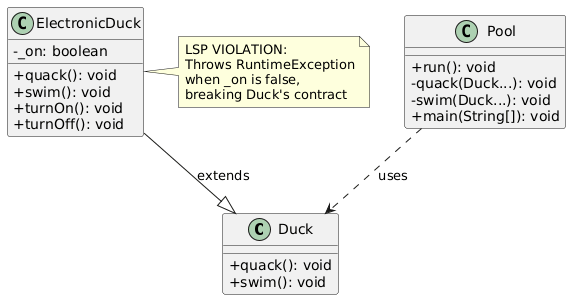
\includegraphics[width=0.8\textwidth]{LSP/plantUML/before.png}
    \caption{UML Diagram - Duck Pool System Before Refactoring (LSP Violation)}
    \label{fig:lsp_before}
\end{figure}

\subsection{Refactored Solution}

\subsubsection{Overview of the Refactoring Approach}

The refactored design eliminates the inheritance relationship and instead uses interface-based composition. The main components are:

\begin{enumerate}
    \item \textbf{IQuackable Interface:} Defines the contract for objects that can quack.
    \item \textbf{ISwimmable Interface:} Defines the contract for objects that can swim.
    \item \textbf{Duck Class:} Implements both interfaces as a regular duck.
    \item \textbf{ElectronicDuck Class:} Implements both interfaces independently, with graceful handling of the off state.
    \item \textbf{Pool Class:} Works with interfaces rather than concrete classes, ensuring proper substitutability.
\end{enumerate}

\subsubsection{Detailed Explanation of Each Component}

\paragraph{IQuackable - Quacking Behavior Contract}

\begin{verbatim}
public interface IQuackable
{
    void quack();
}
\end{verbatim}

\textbf{Design Decision:} Extracted the quacking behavior into a separate interface to define a clear contract without imposing implementation details or inheritance constraints.

\textbf{Responsibility:} Defines the contract for any object that can produce a quacking sound.

\textbf{Reason to change:} Only if the fundamental concept of what it means to quack changes in the domain.

\textbf{Benefits:}
\begin{itemize}
    \item Allows multiple unrelated classes to share quacking behavior without forced inheritance
    \item Provides a clear, minimal contract that's easy to implement correctly
\end{itemize}

\paragraph{ISwimmable - Swimming Behavior Contract}

\begin{verbatim}
public interface ISwimmable
{
    void swim();
}
\end{verbatim}

\textbf{Design Decision:} Extracted the swimming behavior into a separate interface, parallel to IQuackable, to maintain consistent abstraction levels.

\textbf{Responsibility:} Defines the contract for any object capable of swimming.

\textbf{Reason to change:} Only if the fundamental concept of swimming behavior changes in the domain.

\textbf{Benefits:}
\begin{itemize}
    \item Decouples swimming ability from any specific class hierarchy
    \item Enables flexible composition of behaviors
\end{itemize}

\paragraph{Duck - Standard Duck Implementation}

\begin{verbatim}
public class Duck implements IQuackable, ISwimmable
{
    @Override
    public void quack()
    {
        System.out.println("Quack...");
    }

    @Override
    public void swim()
    {
        System.out.println("Swim...");
    }
}
\end{verbatim}

\textbf{Design Decision:} Implements both interfaces to provide standard duck behavior without establishing an inheritance hierarchy.

\textbf{Responsibility:} Represents a biological duck with natural quacking and swimming abilities.

\textbf{Reason to change:} Only if the behavior of biological ducks needs to be modified.

\textbf{Benefits:}
\begin{itemize}
    \item Simple, straightforward implementation with no conditional logic
    \item No longer serves as a base class, avoiding inheritance-related LSP issues
\end{itemize}

\paragraph{ElectronicDuck - Electronic Duck Implementation}

\begin{verbatim}
public class ElectronicDuck implements IQuackable, ISwimmable
{
    private boolean _on = false;

    @Override
    public void quack()
    {
        if (_on) {
            System.out.println("Electronic duck quack...");
        } else {
            System.out.println("...");  // Silent when off
        }
    }

    @Override
    public void swim()
    {
        if (_on) {
            System.out.println("Electronic duck swim");
        } else {
            System.out.println("...");  // Does nothing when off
        }
    }

    public void turnOn()
    {
        _on = true;
    }

    public void turnOff()
    {
        _on = false;
    }
}
\end{verbatim}

\textbf{Design Decision:} Instead of throwing exceptions when powered off, the ElectronicDuck now handles the off state gracefully by doing nothing (printing "..."), which maintains the contract that these methods can always be called safely.

\textbf{Responsibility:} Represents an electronic toy duck that requires power to function and handles its state internally.

\textbf{Reason to change:} Only if the behavior of electronic ducks or their power management needs modification.

\textbf{Benefits:}
\begin{itemize}
    \item No longer throws exceptions, making it safe to use polymorphically
    \item Maintains the contract established by the interfaces
    \item Can be substituted for any IQuackable or ISwimmable without breaking client code
\end{itemize}

\paragraph{Pool - Client Class}

\begin{verbatim}
public class Pool
{
    public void run()
    {
        Duck donaldDuck = new Duck();
        ElectronicDuck electricDuck = new ElectronicDuck();
        electricDuck.turnOn();  // Turn on before using
        
        quack(donaldDuck, electricDuck);
        swim(donaldDuck, electricDuck);
    }

    private void quack(IQuackable... quackables)
    {
        for (IQuackable quackable : quackables) {
            quackable.quack();
        }
    }

    private void swim(ISwimmable... swimmables)
    {
        for (ISwimmable swimmable : swimmables) {
            swimmable.swim();
        }
    }

    public static void main(String[] args)
    {
        Pool pool = new Pool();
        pool.run();
    }
}
\end{verbatim}

\textbf{Design Decision:} Modified to work with interfaces (IQuackable and ISwimmable) instead of concrete Duck class, enabling proper polymorphism.

\textbf{Responsibility:} Manages and coordinates the behavior of objects that can quack and swim.

\textbf{Reason to change:} Only if the pool's coordination logic needs to change.

\textbf{Benefits:}
\begin{itemize}
    \item Depends on abstractions rather than concrete implementations
    \item Can work with any implementation of IQuackable or ISwimmable
    \item Safe from runtime exceptions due to LSP compliance
\end{itemize}

\subsubsection{UML Diagram of the Refactored Design}

\begin{figure}[H]
    \centering
    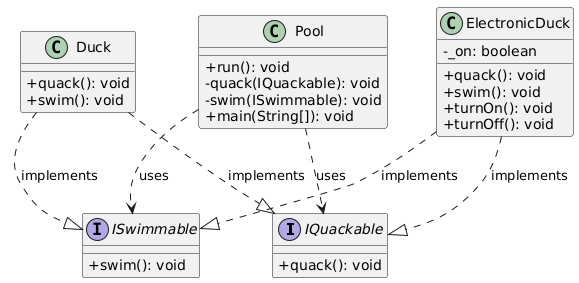
\includegraphics[width=0.95\textwidth]{LSP/plantUML/after.png}
    \caption{UML Diagram - Duck Pool System After Refactoring (LSP Compliant)}
    \label{fig:lsp_after}
\end{figure}

\subsection{How the Refactoring Aligns with LSP}

\subsubsection{Proper Substitutability}

The refactored design ensures that any implementation of IQuackable or ISwimmable can be used interchangeably without breaking the client code:

\begin{table}[H]
\centering
\begin{tabular}{|l|p{8cm}|}
\hline
\textbf{Type} & \textbf{Substitutability Guarantee} \\
\hline
IQuackable & Any implementation can be called with quack() without exceptions or unexpected behavior \\
\hline
ISwimmable & Any implementation can be called with swim() without exceptions or unexpected behavior \\
\hline
Duck & Implements both interfaces with consistent, predictable behavior \\
\hline
ElectronicDuck & Implements both interfaces with graceful degradation when powered off, maintaining contract \\
\hline
\end{tabular}
\caption{LSP Substitutability Analysis}
\label{tab:lsp_substitutability}
\end{table}

\subsubsection{Contract Preservation}

The refactored design preserves behavioral contracts at multiple levels:

\begin{itemize}
    \item \textbf{No Exception Violations:} ElectronicDuck no longer throws RuntimeException when methods are called. Instead, it handles the off state gracefully, maintaining the contract that interface methods can always be invoked safely.
    
    \item \textbf{Precondition Compliance:} Neither Duck nor ElectronicDuck strengthens the preconditions of the interface methods. Both implementations can be called at any time without requiring special initialization from the client's perspective.
    
    \item \textbf{Postcondition Maintenance:} All implementations fulfill the postconditions implied by their interfaces—when quack() is called, some quacking behavior occurs (even if silent for powered-off electronic ducks).
    
    \item \textbf{Behavioral Transparency:} The Pool class can work with any IQuackable or ISwimmable implementation without needing to know which concrete type it's dealing with, demonstrating true substitutability.
\end{itemize}

\subsubsection{Improved Design Quality}

\begin{itemize}
    \item \textbf{Elimination of Inheritance Problems:} By removing the inheritance relationship between Duck and ElectronicDuck, we've eliminated the source of LSP violations. The "is-a" relationship was conceptually flawed—an electronic duck is not truly a substitutable type of duck.
    
    \item \textbf{Interface Segregation:} The use of small, focused interfaces (IQuackable, ISwimmable) ensures that implementations only commit to behaviors they can properly support.
    
    \item \textbf{Composition over Inheritance:} The refactored design favors composition and interface implementation over class inheritance, providing greater flexibility and avoiding LSP pitfalls.
\end{itemize}

\subsection{Conclusion}

The refactoring of the Duck Pool System demonstrates the critical importance of the Liskov Substitution Principle in creating robust, maintainable object-oriented designs. The transformation from an inheritance-based hierarchy to an interface-based composition approach has yielded significant improvements:

\begin{itemize}
    \item \textbf{Elimination of Runtime Exceptions:} The system no longer crashes when ElectronicDuck objects are used polymorphically, making it safer and more reliable.
    
    \item \textbf{True Polymorphic Behavior:} Client code (Pool) can now work with any duck-like object through interfaces without worrying about implementation details or special cases.
    
    \item \textbf{Enhanced Flexibility:} New types of ducks or quackable/swimmable objects can be added by simply implementing the relevant interfaces without affecting existing code.
    
    \item \textbf{Improved Maintainability:} The clear separation of concerns and contract-based design makes the system easier to understand, test, and modify.
    
    \item \textbf{Better Testability:} Mock implementations of IQuackable and ISwimmable can be easily created for testing purposes without the complications of inheritance hierarchies.
\end{itemize}

This exercise illustrates that proper application of LSP often requires reconsidering inheritance relationships and favoring composition with well-defined interfaces. The principle serves as a guardian against misuse of inheritance and ensures that polymorphism delivers on its promise of transparent substitutability.

% ============================================
% SECTION: INTERFACE SEGREGATION PRINCIPLE
% ============================================

\section{Interface Segregation Principle (ISP)}

\subsection{Definition of ISP}

The Interface Segregation Principle was introduced by Robert C. Martin as part of the SOLID principles. It states:

\textit{"No client should be forced to depend on methods it does not use. Interfaces belong to clients, not to hierarchies."}

In practical terms, this means that large, "fat" interfaces should be split into smaller, more specific ones so that implementing classes only need to be concerned with the methods that are relevant to them. This prevents classes from being forced to implement methods they don't need.

\subsection{Importance of ISP in Object-Oriented Design}

The Interface Segregation Principle is essential for creating focused, cohesive abstractions that don't burden their clients with unnecessary dependencies:

\begin{itemize}
    \item \textbf{Reduced Coupling:} By depending only on the methods they actually use, clients are less affected by changes to unrelated functionality, leading to more loosely coupled systems.
    
    \item \textbf{Improved Maintainability:} Smaller, focused interfaces are easier to understand, implement, and maintain than large, monolithic ones. Changes to one aspect of functionality don't ripple through unrelated code.
    
    \item \textbf{Enhanced Flexibility:} Classes can implement multiple small interfaces based on their actual capabilities, rather than being forced into a rigid hierarchy with irrelevant methods.
    
    \item \textbf{Better Testability:} Focused interfaces make it easier to create mock objects and test doubles, as test implementations only need to provide the specific methods being tested.
    
    \item \textbf{Clearer Intent:} Small, role-specific interfaces communicate design intent more clearly than large interfaces, making the system's architecture more comprehensible.
\end{itemize}

\subsection{Exercise Analysis: Smart Door System}

\subsubsection{Description of the Original Design (Before Refactoring)}

The original system models a smart door control system with different types of doors that respond to various stimuli. The design consists of:

\begin{enumerate}
    \item \textbf{Door Interface:} A large interface containing all possible door operations including basic operations (lock, unlock, open, close) and callback methods for different trigger types (timeOutCallback, proximityCallback).
    
    \item \textbf{TimedDoor Class:} A door implementation that responds to timer events by automatically locking after a timeout period. It implements the Door interface but only uses the timer-related callback.
    
    \item \textbf{SensingDoor Class:} A door implementation that responds to proximity sensors by opening when someone approaches. It implements the Door interface but only uses the proximity-related callback.
    
    \item \textbf{Timer Class:} Manages timer events and triggers the timeOutCallback on registered Door objects.
    
    \item \textbf{Sensor Class:} Manages proximity detection and triggers the proximityCallback on registered Door objects.
\end{enumerate}

\subsubsection{Identified ISP Violations}

The original design violates the Interface Segregation Principle in several significant ways:

\begin{itemize}
    \item \textbf{Fat Interface:} The Door interface contains six methods, but no single implementation needs all of them. This forces implementing classes to deal with methods they don't use.
    
    \item \textbf{Forced Stub Implementations:} TimedDoor throws NotImplementedException for proximityCallback(), and SensingDoor throws NotImplementedException for timeOutCallback(). These stub implementations indicate that the classes are being forced to implement methods they cannot meaningfully support.
    
    \item \textbf{Client Confusion:} The Timer and Sensor classes depend on the entire Door interface even though they each only use one method (timeOutCallback and proximityCallback respectively). This creates unnecessary coupling to methods they never invoke.
    
    \item \textbf{Violation of Role Segregation:} The Door interface conflates multiple distinct roles—basic door operations, timer client, and proximity sensor client—into a single monolithic interface. This violates the principle that interfaces should represent cohesive roles.
    
    \item \textbf{Maintenance Burden:} Adding new callback types to the Door interface would force all existing door implementations to provide stub implementations, even if they don't support the new functionality.
\end{itemize}

\subsubsection{UML Diagram of the Original Design}

\begin{figure}[H]
    \centering
    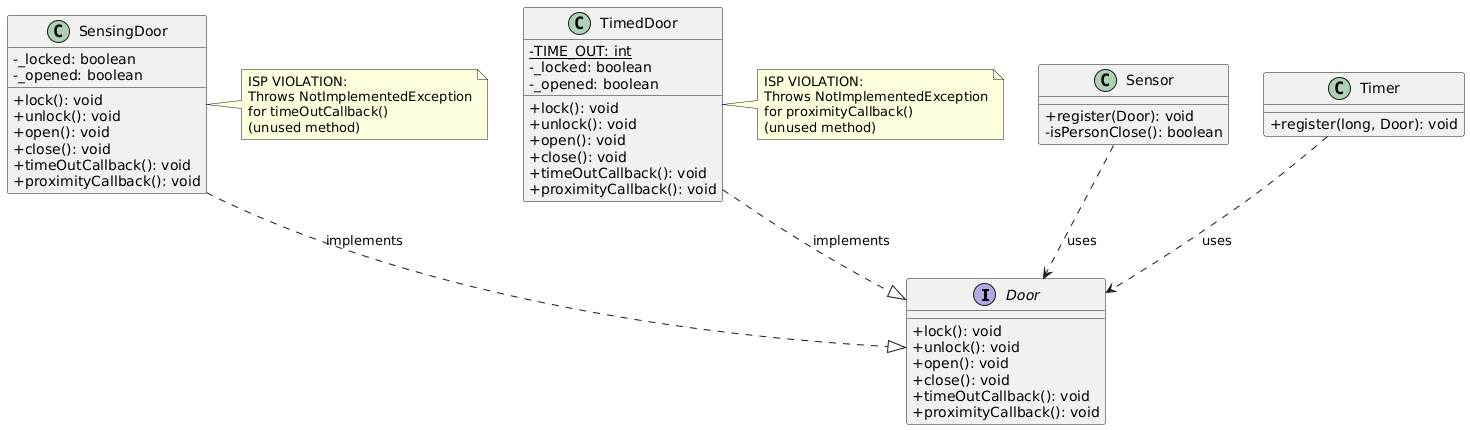
\includegraphics[width=0.8\textwidth]{ISP/plantUML/before.png}
    \caption{UML Diagram - Smart Door System Before Refactoring (ISP Violation)}
    \label{fig:isp_before}
\end{figure}

\subsection{Refactored Solution}

\subsubsection{Overview of the Refactoring Approach}

The refactored design segregates the monolithic Door interface into three focused, role-based interfaces. The main components are:

\begin{enumerate}
    \item \textbf{Door Interface:} Contains only core door operations (lock, unlock, open, close).
    \item \textbf{TimedDoorClient Interface:} Defines the contract for doors that respond to timer events.
    \item \textbf{ProximityDoorClient Interface:} Defines the contract for doors that respond to proximity sensors.
    \item \textbf{TimedDoor Class:} Implements Door and TimedDoorClient, providing timer-responsive behavior.
    \item \textbf{SensingDoor Class:} Implements Door and ProximityDoorClient, providing proximity-responsive behavior.
    \item \textbf{Timer and Sensor Classes:} Depend only on their respective client interfaces.
\end{enumerate}

\subsubsection{Detailed Explanation of Each Component}

\paragraph{Door - Core Door Operations}

\begin{verbatim}
public interface Door
{
    void lock();
    void unlock();
    void open();
    void close();
}
\end{verbatim}

\textbf{Design Decision:} Extracted only the fundamental door operations into this interface, removing all callback methods to create a focused contract for basic door behavior.

\textbf{Responsibility:} Defines the essential operations that all doors must support—locking, unlocking, opening, and closing.

\textbf{Reason to change:} Only if the fundamental concept of door operations changes in the domain.

\textbf{Benefits:}
\begin{itemize}
    \item Provides a clean, minimal contract that any door can implement
    \item Can be implemented without any stubs or NotImplementedException
\end{itemize}

\paragraph{TimedDoorClient - Timer Event Handler}

\begin{verbatim}
public interface TimedDoorClient
{
    void timeOutCallback();
}
\end{verbatim}

\textbf{Design Decision:} Created a separate interface specifically for objects that respond to timer events, following the principle that interfaces should represent distinct client roles.

\textbf{Responsibility:} Defines the contract for objects that can receive and handle timeout notifications.

\textbf{Reason to change:} Only if the timer callback mechanism needs to be modified.

\textbf{Benefits:}
\begin{itemize}
    \item Allows only timer-aware components to implement this interface
    \item Provides clear semantic meaning—implementers are timer clients
\end{itemize}

\paragraph{ProximityDoorClient - Proximity Event Handler}

\begin{verbatim}
public interface ProximityDoorClient
{
    void proximityCallback();
}
\end{verbatim}

\textbf{Design Decision:} Created a separate interface specifically for objects that respond to proximity sensor events, parallel to TimedDoorClient.

\textbf{Responsibility:} Defines the contract for objects that can receive and handle proximity detection notifications.

\textbf{Reason to change:} Only if the proximity callback mechanism needs to be modified.

\textbf{Benefits:}
\begin{itemize}
    \item Allows only proximity-aware components to implement this interface
    \item Clearly communicates that implementers respond to proximity events
\end{itemize}

\paragraph{TimedDoor - Timer-Responsive Door}

\begin{verbatim}
public class TimedDoor implements Door, TimedDoorClient
{
    private static final int TIME_OUT = 100;
    private boolean _locked;
    private boolean _opened;

    public TimedDoor(Timer timer)
    {
        timer.register(TIME_OUT, this);
    }

    @Override
    public void lock()
    {
        _locked = true;
    }

    @Override
    public void unlock()
    {
        _locked = false;
    }

    @Override
    public void open()
    {
        if (!_locked) {
            _opened = true;
        }
    }

    @Override
    public void close()
    {
        _opened = false;
    }

    @Override
    public void timeOutCallback()
    {
        _locked = true;
    }
}
\end{verbatim}

\textbf{Design Decision:} Implements both Door and TimedDoorClient interfaces, but not ProximityDoorClient, accurately reflecting its actual capabilities.

\textbf{Responsibility:} Represents a door that automatically locks itself after a timeout period.

\textbf{Reason to change:} Only if the behavior of timer-based locking needs to be modified.

\textbf{Benefits:}
\begin{itemize}
    \item No longer forced to implement proximityCallback()
    \item No NotImplementedException needed—all implemented methods are meaningful
    \item Clear declaration of supported functionality through interface selection
\end{itemize}

\paragraph{SensingDoor - Proximity-Responsive Door}

\begin{verbatim}
public class SensingDoor implements Door, ProximityDoorClient
{
    private boolean _locked;
    private boolean _opened;

    public SensingDoor(Sensor sensor)
    {
        sensor.register(this);
    }

    @Override
    public void lock()
    {
        _locked = true;
    }

    @Override
    public void unlock()
    {
        _locked = false;
    }

    @Override
    public void open()
    {
        if (!_locked) {
            _opened = true;
        }
    }

    @Override
    public void close()
    {
        _opened = false;
    }

    @Override
    public void proximityCallback()
    {
        _opened = true;
    }
}
\end{verbatim}

\textbf{Design Decision:} Implements both Door and ProximityDoorClient interfaces, but not TimedDoorClient, accurately reflecting its actual capabilities.

\textbf{Responsibility:} Represents a door that automatically opens when someone approaches.

\textbf{Reason to change:} Only if the behavior of proximity-based opening needs to be modified.

\textbf{Benefits:}
\begin{itemize}
    \item No longer forced to implement timeOutCallback()
    \item No NotImplementedException needed—all implemented methods are meaningful
    \item Clear declaration of supported functionality through interface selection
\end{itemize}

\paragraph{Timer - Timer Event Manager}

\begin{verbatim}
public class Timer
{
    public void register(long timeOut, final TimedDoorClient client)
    {
        java.util.Timer timerUtility = new java.util.Timer();
        timerUtility.schedule(new TimerTask()
        {
            @Override
            public void run()
            {
                client.timeOutCallback();
            }
        }, timeOut);
    }
}
\end{verbatim}

\textbf{Design Decision:} Changed to depend on TimedDoorClient interface instead of the full Door interface, reducing unnecessary coupling.

\textbf{Responsibility:} Manages timer events and notifies registered clients when timeouts occur.

\textbf{Reason to change:} Only if timer management logic needs modification.

\textbf{Benefits:}
\begin{itemize}
    \item Depends only on the timeOutCallback() method it actually uses
    \item Can work with any TimedDoorClient, not just doors
    \item Reduced coupling to unrelated door operations
\end{itemize}

\paragraph{Sensor - Proximity Detection Manager}

\begin{verbatim}
public class Sensor
{
    public void register(ProximityDoorClient client)
    {
        while (true) {
            if (isPersonClose()) {
                client.proximityCallback();
                break;
            }
        }
    }

    private boolean isPersonClose()
    {
        return new Random().nextBoolean();
    }
}
\end{verbatim}

\textbf{Design Decision:} Changed to depend on ProximityDoorClient interface instead of the full Door interface, reducing unnecessary coupling.

\textbf{Responsibility:} Detects proximity events and notifies registered clients.

\textbf{Reason to change:} Only if proximity detection logic needs modification.

\textbf{Benefits:}
\begin{itemize}
    \item Depends only on the proximityCallback() method it actually uses
    \item Can work with any ProximityDoorClient, not just doors
    \item Reduced coupling to unrelated door operations
\end{itemize}

\subsubsection{UML Diagram of the Refactored Design}

\begin{figure}[H]
    \centering
    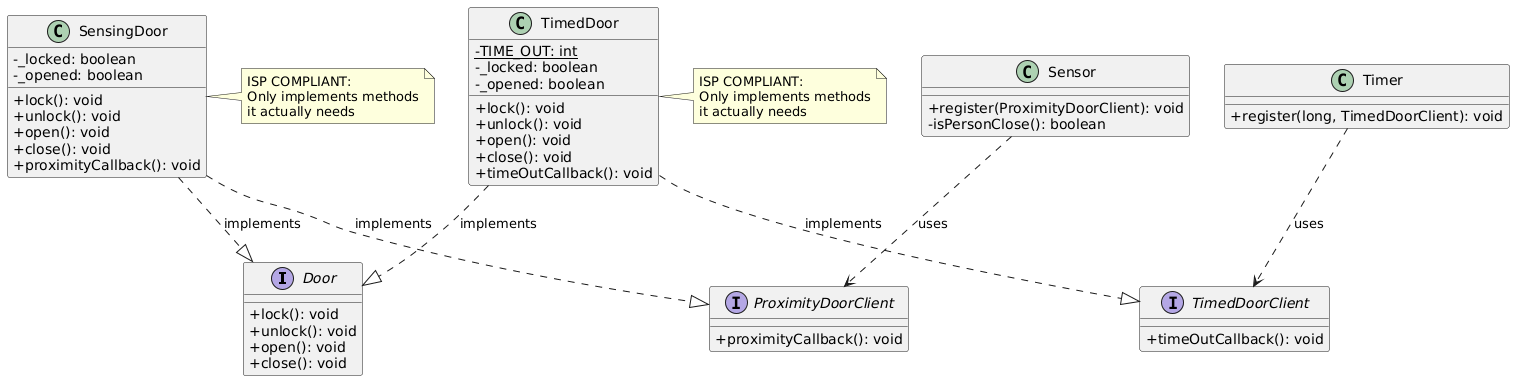
\includegraphics[width=0.95\textwidth]{ISP/plantUML/after.png}
    \caption{UML Diagram - Smart Door System After Refactoring (ISP Compliant)}
    \label{fig:isp_after}
\end{figure}

\subsection{How the Refactoring Aligns with ISP}

\subsubsection{Interface Segregation by Client Role}

The refactored design properly segregates interfaces based on distinct client roles:

\begin{table}[H]
\centering
\begin{tabular}{|l|p{4cm}|p{5cm}|}
\hline
\textbf{Interface} & \textbf{Client Type} & \textbf{Methods Used} \\
\hline
Door & General door users & lock(), unlock(), open(), close() \\
\hline
TimedDoorClient & Timer system & timeOutCallback() \\
\hline
ProximityDoorClient & Proximity sensor system & proximityCallback() \\
\hline
\end{tabular}
\caption{ISP Interface-Client Mapping}
\label{tab:isp_interface_clients}
\end{table}

\subsubsection{Elimination of Forced Dependencies}

The refactoring has eliminated all forced dependencies and stub implementations:

\begin{itemize}
    \item \textbf{No NotImplementedException:} Neither TimedDoor nor SensingDoor needs to throw NotImplementedException because they only implement interfaces for functionality they actually support.
    
    \item \textbf{Precise Interface Implementation:} Each class implements only the interfaces that match its capabilities:
    \begin{itemize}
        \item TimedDoor implements Door + TimedDoorClient
        \item SensingDoor implements Door + ProximityDoorClient
    \end{itemize}
    
    \item \textbf{Focused Client Dependencies:} Timer and Sensor classes depend only on the specific callback interfaces they need, not on the entire Door interface with its irrelevant methods.
    
    \item \textbf{Flexibility for Future Extensions:} New door types can be added by implementing only the interfaces they need. For example, a SimpleDoor could implement only the Door interface without any callbacks.
\end{itemize}

\subsubsection{Improved Cohesion and Reduced Coupling}

\begin{itemize}
    \item \textbf{High Interface Cohesion:} Each interface represents a single, well-defined responsibility. The Door interface handles door operations, TimedDoorClient handles timer events, and ProximityDoorClient handles proximity events.
    
    \item \textbf{Reduced Coupling:} Clients are coupled only to the specific abstractions they need. The Timer doesn't know about proximity callbacks, and the Sensor doesn't know about timeout callbacks.
    
    \item \textbf{Clear Semantic Boundaries:} The separation of interfaces creates clear semantic boundaries in the system. Each interface name clearly communicates its purpose and the role of its implementers.
    
    \item \textbf{Easier Testing:} Mock implementations for testing are simpler to create because test doubles only need to implement the specific interface being tested, not a large monolithic interface.
\end{itemize}

\subsection{Conclusion}

The refactoring of the Smart Door System demonstrates how the Interface Segregation Principle leads to more flexible, maintainable, and understandable code. The transformation from a single fat interface to multiple focused interfaces has produced significant improvements:

\begin{itemize}
    \item \textbf{Elimination of Stub Implementations:} The removal of NotImplementedException and dummy implementations makes the code cleaner and more honest about what each class can actually do.
    
    \item \textbf{Precise Dependency Management:} Each component depends only on the methods it actually uses, reducing unnecessary coupling and making the system more resilient to change.
    
    \item \textbf{Clearer Design Intent:} The use of role-specific interfaces clarifies the design intent and makes it easier for developers to understand the responsibilities of each class.
\end{itemize}